\chapter{Methods}\label{cha:Methods}
\section{Distance Function}
\subsection{Motivation}\label{sub:Motivation}
In section \ref{loss_landscape}, we got a brief overview over the loss landscape
of deep neural networks and the resulting challenges for optimization. Although
there exist a large number of local minima, most of them have low cost.
Furthermore, they are arranged in cells, where each minima has low cost and is
connected to the others via valleys of low loss.

These cells create a challenge for optimization. Suppose the learning gets into
the area of one of these cells. As mentioned in chapter \ref{loss_landscape} the
cells are surrounded by nondifferential boundaries and areas of higher loss.
This will likely cause the algorithm to get stuck into this cell. As all of the
connected minimas in this cell are of approximatly same loss, there will be a
boundary until the algorithm can improve, which may be higher than the global
optimum. This imposes the question, if continuing to train is useful, as after
one of the minima of the cell is found, the nearby minima it can reach will
offer no significant improvement and other cells are out of reach.

If we reuse the ball analogy from section \ref{sub:Momentum}, the beginning of
the training process would probably place the ball at the top of a mountain
landscape. The initial training let's the ball move into one of the valleys.
This valley may connect the ball to other points of low altitude, like minima
are connected in a cell. When the ball is only allowed to move downhill however,
the ball can never reach a spot which he is seperated by a hill. Thus, his
minimum altitude is bound to the lowest place in his current valley. If we add
momentum, we have seen that the ball is able to get over hills of certain size
by using his momentum. Warm restarts add the possibility to jump over a hill
with a high learning rate at each restart. This can lead to an escape of the
cell, but without guarantee. What is more likely to happen is that after a large
step, the ball is in an area of higher altitude, which will let him roll down to
the same valley again in the next step.

In contrast, we try a different approach. Rather than letting the ball make one
large steps and then allowing him to move on freely, we want to constantly push
the ball away from it's current position. The idea beeing if the ball is only
surrounded by hills, we have to push it up one of these until it reaches the top
and can then roll down into another valley, therefore escaping the cell.
Transferred back to a real network, this translates to repeatedly updating the
parameter values in a way, that the new values will increase their distance to
the values we want to get away from.


\begin{algorithm}\label{alg:Distance_Motivation}
    \begin{algorithmic}[1]
        \caption{Machine Learning with distancing}
        \REQUIRE a set of parameters $\theta$ and a dataset
        \ENSURE a assignment of $\theta$ which maximizes performance
        \STATE initialize the network, dataset and training parameters
        \FOR{$i \leftarrow 1$ \textbf{to} desired number of epochs}
            \STATE compute foward and backward pass of training data
            \STATE update parameter values with optimizer
        \ENDFOR
        \STATE create checkpoint we want to distance from
		\FOR{$i \leftarrow$ next epoch \textbf{to} end}
			\FOR{checkpoint \textbf{in} list of checkpoints}
			\STATE compute parameter update which increases the distance to checkpoint
			\ENDFOR
		\STATE update parameter values with optimizer
        \ENDFOR
        \STATE \textbf{return: the final assignment of $\theta$}
    \end{algorithmic}
\end{algorithm}

Algorithm \ref{alg:Distance_Motivation} shows the formalization of the idea into
pseudo-code. First, we train the network the traiditional way - we compute the
foward and backward pass of the training data with the resulting gradient, and
then update the parameter values with an optimizer. After we have reached a
sufficiently low error, we create the point we want to push away from, which we
call \textbf{checkpoint}. The difference in the next training loop in contrast
to the standard one at the beginning is how the parameter values are computed.
Here, our goal is to distance from the checkpoint. This will also result in a
gradient, which will be applied the same way as above.

How can we encourage a network to distance from a checkpoint, while at the same
time not sacrificing the networks performance? Back to the ball analogy, instead
of pushing the ball up a hill, we could place a hill at the current position,
and let the ball roll down. Figure \ref{fig:Distance2D} shows a graphical
illustration for the 2D case. The function $f(x)$ has a local minimum, where an
algorithm might get stuck. If we add a gaussian curve $g(x)$ with the maximum
aligned to the minimum of $f(x)$, we can see that the minimum disappears. An
advantage of this technique is that the hill will only change the loss landscape
locally. So when we have distanced from the hill, we follow the normal loss
landscape again.

\begin{figure}[h!]\label{fig:Distance2D}
    \begin{center}
        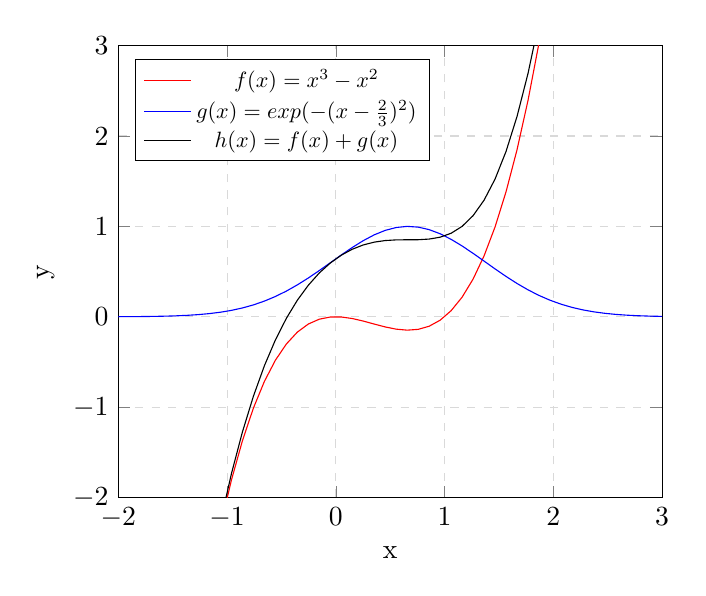
\begin{tikzpicture}
            \begin{axis}[
            grid=major, 
            grid style={dashed,gray!30},
            xlabel=x, % Set the labels
            ylabel=y,
            xmin=-2,
            xmax=3,
            xtick={-2,-1,0,1,2, 3},
            ymin=-2,
            ymax=3,
            samples=100,
            legend pos = north west,
            width=0.7\textwidth,
            legend style={nodes={scale=0.8, transform shape}}]
            \addplot[color=red]{x^3-x^2};
            \addlegendentry{$f(x)=x^3-x^2$}
            \addplot[color=blue]{exp(-(x-2/3)^2)};
            \addlegendentry{$g(x)=exp(-(x-\frac{2}{3})^2)$}
            \addplot[color=black]{x^3-x^2+exp(-(x-2/3)^2)};
            \addlegendentry{$h(x)=f(x)+g(x)$}
            \end{axis}
         \end{tikzpicture}
        \caption{Example of a function with a local minimum at $x=\frac{2}{3}$. If we place an Gaussian function on top, the minimum disappears. Note, that the black function approaches the red if we distance from the local minimum.}
    \end{center}
\end{figure}

Formally, this hill is realised by first computing the distance of the parameter
values to the checkpoint, and then adding a penalty for small distances. If we
use and exponential Kernel, the idea of the hill can be taken quite visually.
Section \ref{sub:Mathematical_approach} describes the mathematical approach in
detail.

What happens when our penalty hill is not large enough to get the ball over the
hill? This means we would get back to the present parameter values. That's not
necesarryly a problem, as it would mean that our current position is very
robust, which would lead to a good generalization capability. Therefore our
network would stay in areas with stable minima, which is a desired property.

For ensemble methods, there are other possible benefits of this approach. Recall
that for an ensemble to perform well, the errors of the participating networks
should be uncorellated. SGD with warm restart \cite{loshchilov2016sgdr} tried to
ensure this with warm restarts, where a high learnin rate increases the distance
of the networks and therefore leads to uncorellated errors. We could use our
method as alternative approach, where we ensure the distance between the
networks not only by high learning rate but by explicitly increasing the
distance. Of course, the underlying idea for both is that networks which are
more distant in parameter space will behave more differently, and therefore have
more uncorellated errors.



\subsection{Mathematical approach}\label{sub:Mathematical_approach}
\subsubsection{Distance function}\label{distance_function}
As we want to measure the distance between two points, we need to define a
distance function. A common choice is the euclidean distance also know as $L_2$
norm, which is defined as: 
\begin{align}
    \rVert x \lVert_2 = \sqrt{\sum_i \lvert x_i \rvert^2}
\end{align}
This norm can also be squared to get rid of the root. Squaring does not change
the direction of the gradient, and is therefore possible. To measure the
distance between two parameter states $\theta_1$ and $\theta_2$ of the networks,
this results in:
\begin{align}\label{eq:distance}
    L_2 (\theta_1, \theta_2)= \sum_i (\theta_{1_i}-\theta_{2_i})^2
\end{align}
The size and shape of the paramters $\theta$ is not important, as each paramter
is only compared to another state of itself, and is combined via a sum.

An undesireable property of the current formulation is that the values the
distance function can take is partly dependend on the size of the network.
Consider two networks $\theta_1$, $\theta_2$ with the same classification task,
but the number of parameters of $\theta_1$ is larger than $\theta_2$ If we
assume all of the parameters are distributed the same way, then $\theta_1$ would
output a larger distance than $\theta_2$. However it would be desirable for the
functions to be in the same bound, as it would make the transfer of
hyperparameters for example possible. That's why we need a function to let the
output stay in a certan bound.

If we take a look at support vector machines, they use kernels to compute the
similarity between two samples. One popular choice is the radial basis function
kernel, defined as:
\begin{align}\label{eq:RBF}
    k(\theta_1, \theta_2)=exp(-\frac{\rVert \theta_1 - \theta_2 \lVert^2}{\sigma^2})
\end{align}
where $exp$ is the exponential function. With the use of \ref{eq:distance}, we
can convert this to:
\begin{align}\label{eq:DistanceFinal}
    distance(\theta_1, \theta_2)=exp(-\frac{L_2 (\theta_1, \theta_2)}{\sigma^2})
\end{align}

If we plot this function in the two dimensional case in figure
\ref{fig:Gaussian}, we can see some nice properties. First of all, the values
are now bound between 0 an 1, regardless of the size of $\theta$. Second, we can
see as the values of the distance get larger, the function approaches 0
asymtotically. This leads to a really small gradient for extreme distances.
Consequently, the Kernel will initially push the parameters away from the
checkpoint, but when this is achieved, will have little influence on the loss
function. How far the function encourages to distance from the checkpoint can be
controlled by the parameter $\sigma$, which defines the width of the function
and can be tuned as a hyperparamter. As $\sigma$ gets larger, the function
becomes wider. Therefore, the influence of the distance function will reach
further the larger $\sigma$ is.

\begin{figure}[h]\label{fig:Gaussian}
    \centering
    \begin{center}
        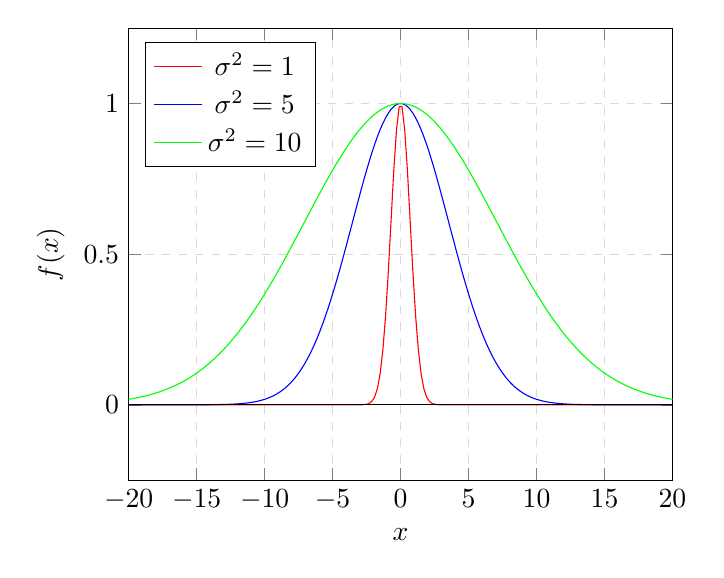
\begin{tikzpicture}
            \begin{axis}[
            grid=major, 
            grid style={dashed,gray!30},
            xlabel=$x$, % Set the labels
            ylabel=$f(x)$,
            xmin=-20,
            xmax=20,
            xtick={-20,-15,-10,-5,0,5,10,15,20},
            ytick={0,0.5,1},
            ymin=-0.25,
            ymax=1.25,
            samples=200,
            legend pos = north west,
            width=0.7\textwidth,
            legend style={nodes={scale=1, transform shape}},
            domain=-20:20]
            \addplot[color=red]{exp(-x^2)};
            \addlegendentry{$\sigma^2=1$}
            \addplot[color=blue]{exp(-x^2/5^2)};
            \addlegendentry{$\sigma^2=5$}
            \addplot[color=green]{exp(-x^2/10^2)};
            \addlegendentry{$\sigma^2=10$}
            \addplot[color=black]{0};
            \end{axis}
         \end{tikzpicture}
         \caption{Plot of the function $f(x)=exp(-\frac{x^2}{\sigma^2})$ for different values of $\sigma^2$.}
    \end{center}
\end{figure}


\subsubsection{Loss function}\label{sub:Loss_function}
The last section has focused on how to implement a loss function which achieves
distancing from parameter values. However, only using this loss function would
sacrafice network performance. Therefore, we combine it with the standard loss
function of the task. The state of the art loss function for image
classification, which will be used for testing later, is the cross-entropy-loss
defined as:
\begin{align}
    -\sum_{i} \delta_{yc} log(f(x)_i)
\end{align}
Where $\delta$ is the Kronecker-Delta function defined as:
\begin{align}
    \delta_{xy} =
    \begin{cases}
        1 \textrm{, if } x=y \\
        0 \textrm{ otherwise}
    \end{cases}
\end{align}

To account for the distance term, we just sum it with the cross-entropy-loss:
\begin{align}\label{eq:Loss_distance}
    L=\sum_{i} \delta_{yi} log(f(x)_i) + distance(\theta, \theta_c)
\end{align}
Where $\theta_c$ is the checkpoint. Note that we can do this multiple times, so
we can incooperate multiple checkpoints. Here, we divide by the number of
checkpoints to keep the influence of the distance function on the loss function
irrelevant of the number of checkpoints.
\begin{align}
    L=\sum_{i} \delta_{yi} log(f(x)_i) + \frac{1}{c} \sum_c distance(\theta, \theta_c)
\end{align}
When computing the derivative for the backpropagation, the sum
decomposes into two terms, so the cross-entropy-loss will be computed the same
as before. Another property we want to control for is the influence of the
distance versus the cross-entropy-loss. When training is in later stages, the
cross-entropy-loss may be very small. If the values of the distance function a
too large in comparison, this would cause the parameters to be updated only
based on the distance, which is undesirable as the performance wouldn't be taken
into account anymore. The same is also true the other way around, if the
distance function is too small, it wouldn't affect training at all. That's why
we introduce a hyperparameters $s$ called strength to control this:
\begin{align}\label{eq:Loss_strength}
    L=\sum_{c} \delta_{yc} log(f(x)_c) + s \cdot distance(\theta, \theta_c)
\end{align}
Figure \ref{fig:Gaussian_strength} shows the infuence of $s$ on the distance
function. The values are now bound between 0 and $s$. Increasing the strength
also has the same effect of the function getting wider as in figure
\ref{fig:Gaussian}, but at a much smaller scale. 

\begin{figure}[h]\label{fig:Gaussian_strength}
    \centering
    \begin{center}
        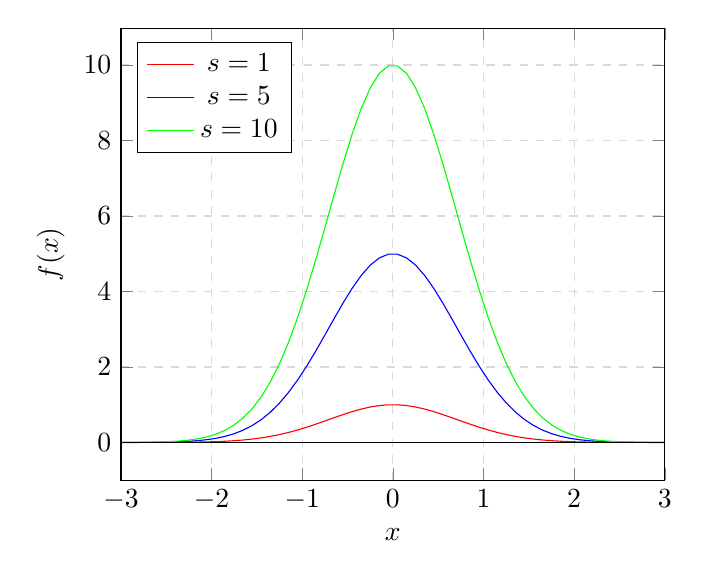
\begin{tikzpicture}
            \begin{axis}[
            grid=major, 
            grid style={dashed,gray!30},
            xlabel=$x$,
            ylabel=$f(x)$,
            xmin=-3,
            xmax=3,
            %xtick={-5,-1,0,1,5},
            %ytick={0,1,5,10},
            %ymin=-1,
            %ymax=11,
            samples=400,
            legend pos = north west,
            width=0.7\textwidth,
            legend style={nodes={scale=1, transform shape}},
            domain=-20:20]
            \addplot[color=red]{exp(-x^2)};
            \addlegendentry{$s=1$}
            \addplot[color=blue]{5*exp(-x^2)};
            \addlegendentry{$s=5$}
            \addplot[color=green]{10*exp(-x^2)};
            \addlegendentry{$s=10$}
            \addplot[color=black]{0};
            \end{axis}
         \end{tikzpicture}
         \caption{Plot of the function $f(x)=s\cdot exp(-\frac{x^2}{\sigma^2})$ for different values of $s$.}
    \end{center}
\end{figure}

Algorithm \ref{alg:Distance_update} shows the full update step. The algorithm is
similar to SGD from \ref{alg:SGD}, only the distance function is added to
compute the gradients.

\begin{algorithm}\label{alg:Distance_update}
    \begin{algorithmic}[1]
        \caption{Update step with distancing}
        \REQUIRE learning rate $\alpha$, distance hyperparameters $s$ and $\sigma$
        \ENSURE a trained neural network
        \STATE initialize the network, dataset and training parameters
        \WHILE{stopping criteria is not met}
            \STATE sample minibatch of $m$ examples ${x^{(1)}, ... ,x^{(n)}}$
            \STATE compute gradient estimate $\hat{g}=\nabla_\theta \frac{1}{m} \sum_i L(f(x^{(i)};\theta),y^{(i)})+s\cdot distance(\theta , \theta_c)$
            \STATE apply parameter update $\theta=\theta-\alpha\cdot\hat{g}$
        \ENDWHILE
        \STATE \textbf{return: the trained network}
    \end{algorithmic}
\end{algorithm}

\subsubsection{Effect on Gradient}\label{sub:Effect_on_Gradient} 
In section \ref{sub:Loss_function}, we showed how the new loss function is
composed. The normal cross-entropy-loss and the distance function are added
together. Therefore, taking the derivative of equation \ref{eq:Loss_distance}
results in 
\begin{align}
    \nabla_\theta L 
    &= \nabla_\theta (\sum_{i} \delta_{yi} log(f(x)_i) + distance(\theta, \theta_c))\\
    &= \nabla_\theta (\sum_{i} \delta_{yi} log(f(x)_i)) + \nabla_\theta distance(\theta, \theta_c)
\end{align}
The derivative of the sum decomposes in the sum of the derivatives. Therefore,
the cross-entropy-loss will be added to the gradient the same as before. The new
term is the distance function on the right.

First of all, it influences the direction of the gradient, so that the network
parameters distance from their checkpoint values. If we take one parameter
$\theta_i$ and compute the derivative of the distance function with respect to
the checkpoint $\theta_c$, we end up with:
\begin{align}
    \nabla_{\theta_i} distance(\theta_c, \theta_i)
    &= \nabla_{\theta_i} exp(-\frac{\sum_j (\theta_{c_j}-\theta_{j})^2}{\sigma^2}) \\
    &= \nabla_{\theta_i} (-\frac{\sum_j (\theta_{c_j}-\theta_{j})^2}{\sigma^2}) \cdot exp(-\frac{\sum_j (\theta_{c_j}-\theta_{j})^2}{\sigma^2}) \\
    &= -\frac{1}{\sigma^2} \cdot \nabla_{\theta_i} \sum_j (\theta_{c_j}-\theta_{j})^2 \cdot exp(-\frac{\sum_j (\theta_{c_j}-\theta_{j})^2}{\sigma^2}) \\
    &= -\frac{1}{\sigma^2} \cdot 2 (\theta_{c_i} - \theta_i) \cdot \nabla_{\theta_i}(\theta_{c_i} - \theta_i) \cdot exp(-\frac{\sum_j (\theta_{c_j}-\theta_{j})^2}{\sigma^2}) \\
    &= -\frac{1}{\sigma^2} \cdot 2 (\theta_{c_i} - \theta_i) \cdot (-1) \cdot exp(-\frac{\sum_j (\theta_{c_j}-\theta_{j})^2}{\sigma^2}) \\
    &= \frac{2}{\sigma^2} \cdot (\theta_{c_i} - \theta_i) \cdot exp(-\frac{\sum_j (\theta_{c_j}-\theta_{j})^2}{\sigma^2}) 
\end{align}

Only the factor $(\theta_{c_i} - \theta_i)$ will affect the direction of the
gradient, the other terms will be $>=0$ for $\forall \theta_i , \theta_{c_i}\in
\mathbb{R}$ and only scale the size. Therefore, they can be disregarded and
there are three cases:
\begin{itemize}
    \item $\theta_{c_i} > \theta_i$\\
        It follows that $\nabla_{\theta_i} distance(\theta_{c_i}, \theta_i)$
        will be positive. As we apply the negative gradient to update the
        parameters, $\theta_i$ will get smaller and  $(\theta_{c_i} - \theta_i)^2$
        will be increase.
    \item $\theta_{c_i} < \theta_i$\\
        $\nabla_{\theta_i} distance(\theta_{c_i}, \theta_i)$ will be negative
        and the distance $(\theta_{c_i} - \theta_i)^2$ will increase the same as
        above.
    \item $\theta_{c_i} = \theta_i$\\
        $\nabla_{\theta_i} distance(\theta_{c_i}, \theta_i)$ will be 0.
        Therefore, the parameter value $\theta_i$ will stay the same.
\end{itemize} 

For $\theta_{c_i} \neq \theta_i$, the gradient of the distance function will
successfully increase the distance. For $\theta_{c_i} = \theta_i$ however, it
will introduce no gradient at all. This would problematic, as when a checkpoint
is created, before the first update this case is true. However, the update is
also composed of the cross-entropy-loss, which will likely introduce an non-zero
gradient. In the next iteration, $\theta_{c_i} \neq \theta_i$ will then be true
and the distance function works as expected. If Momentum is used, there is
another term that prevents the gradient from becoming 0.


Besides the influence of the distance function on the direction of the gradient,
we expect an influence size of the gradient. Assume that the direction of the
gradient is stable across multiple iterations, which is likely if we use
Momentum. After we create a checkpoint, the normal loss function would therefore
increase the distance to the checkpoint by itself. As we have seen above, the
gradient of the distance function will also increase the distance, therefore
both gradients will point in the same direction. For a stable gradient direction
of the normal loss function, the distance function therefore increases the
gradient size rather than change the gradient orientation. Only when the
direction for a parameter changes, the distance term will work against it.

\subsubsection{Computational analysis}\label{sub:Computational_Analysis}
Although the network performance is one of the most important aspects of a
neural network, other factors like training time have to be taken into account.
Here, we will analyze how the distance term affects training time. Algorithm
\ref{alg:Checkpoint} shows that at the beginning, the network is trained as
usual. Therefore, there is no additional training time in this stage. After we
add the checkpoint however, the distance function is added to the loss. In
section \ref{sub:Effect_on_Gradient} we have seen that there is no interaction
between the gradient of the cross-entropy-loss and the distance function. The
same is true for the foward pass. Therefore, the only added computation time
raises from the distance term itself.

The number of parameters of the network stays constant over the epochs.
Therefore, the number of mathematical operations in the foward and backward pass
of the distance term stays constant. Lets assume the comparison time for two
numbers is also constant regardless of their size. Then it follows, that the
distance function creates a constant additional amount of time, denotet by $d$.
In addition, let $l$ denote the constant cost of one pass trough the regular
training loop. If we pass this loop $n$ times, our inital cost is $O(l\cdot
n)=O(n)$. If we add our distance function, we have to add $O(n\cdot d)$ to our
cost $O(n\cdot l + n \cdot d)$. As $O(n\cdot l + n \cdot d)=O(n\cdot (l +
d))=O(n)$, the complexity of the algorithm stays the same. However, the distance
function will still raise the per epoch cost, although by a constant. If we add
more checkpoints, there are again no interactions with other checkpoints or the
regular training loop. Therefore, every new checkpoint should add the same
additional cost, while keeping the complexity class the same. The actual value
of the additional cost will be discussed in the results, section
\ref{Res:Computational_cost}.


\subsection{Pytorch implementation}

\subsubsection{Checkpoint creation}
To measure the distance, we have to create the checkpoint. The model parameters
in pytorch are stored as matrices for each layer and can be accesed via
$model.parameters()$, which outputs an iterable. We therefore opt to keep this
structure and safe the parameters in a list.
\begin{algorithm}[h!]
    \caption{Checkpoint}\label{alg:Checkpoint}
    \lstset{language=Python}
    \lstinputlisting{src/createCheckpoint.py}
\end{algorithm}
\newline
First, the checkpoint list is initialized. Then we iterate over the model
parameters. For each layer, we have to clone the parameters in order to create
new variables, and not just pointers to the existing ones. In addition they have
to be detached, to remove connection of the gradient to the model parameters.

\subsubsection{Distance function}
The L2 norm is implemented the follwing way: We iterate over the checkpoint and
the current parameter values. For each layer, we compute the difference, and
then square and add the values to our distance.
\begin{algorithm}[h!]
    \caption{L2 norm}\label{alg:L2Norm}
    \lstset{language=Python}
    \lstinputlisting{src/L2.py}
\end{algorithm}

\subsubsection{Loss function}
Finally, we add our distance term and the regular loss function together. First,
the standard loss is computed. Then, we iterate over all checkpoints and add
their resulting distance values to the loss.
\begin{algorithm}[h!]
    \caption{Loss function}
    \lstset{language=Python}
    \lstinputlisting{src/loss_distance.py}
\end{algorithm}



\section{Configuration}

\subsection{Library and Training}
The code for the network was written in Python 3.7.4 , with the use of Pytorch
\cite{NEURIPS2019_9015} as the machine learning library. Data that occured
during training was logged and plotted with Tensorboard. Training was done on
the TCML Cluster of the University of Tübingen \cite{TCML}.

\subsection{Dataset}
CIFAR-10 \cite{CIFAR-10} is a popular dataset for image classification. It
consists of 60000 32x32 colour images with 10 different classes. The dataset is
seperated into 50000 train and 10000 test images. The state of the art accuracy
is 97.3\%, reported from Kolesnikov et al. \cite{kolesnikov2019big}.

The data is tranformed by using a random crop, random horizontal flip and
normalization.


\subsection{Networks}
\subsubsection{ResNet}\label{sub:ResNet}
The Residual Network (ResNet) architecture was first proposed by He et al.
\cite{he2016deep}. The idea of the ResNet was, that it is more easy for a
network to learn the residuals rather than the full transformation of an input.
Formally, consider the input $x$. The network transforms $x$ accoring to $H(x)$.
Rather than letting the network do the full transformation, ResNet produces
$H(x)= x +f(x)$, where $f(x)$ is the residual transformation learned by the
network, and x the identity data which is realized by a skip connection. Figure
\ref{fig:Residual_Block} shows a graphical illustration. Beside the assumably
easier to learn representation, ResNet also solves other problems. The issue of
the vanishing gradient as discussed in section \ref{sub:Vanishing_gradient} for
example is tackled, as skip connections backpropagate the gradient better to
earlier layers of the network. This allows for deeper networks.

\begin{figure}[h]\label{fig:Residual_Block}
    \centering
    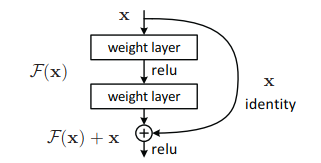
\includegraphics[width=0.6\textwidth]{images/Residual_Block.png}
    \caption{Residual Block from \cite[Page 2]{he2016deep}}
\end{figure}

ResNet creates basic building blocks by applying a convolution, a Relu and
another convolution before adding the skip connection with a final Relu. Figure
\ref{fig:Residual_Block} illustrates this block. The blocks are then stacked
after each other. To let the network learn a more complex representation, after
a number of block, they increase the number of channels. Here, the identity
mapping of the skip connection is replaced by a pointwise convolution to
increase the number of channels. Alternatively, the new channels are padded with
0.



\subsubsection{MobileNetV2}
MobileNet was first introduced by Howard et. al \cite{howard2017mobilenets} as a
lightweight neural network for the use on mobile devices. To reduce the
computation effort of the network, they made use of the depth-wise seperable
convolution. Consider a 32x32x3 image of the CIFAR-10 dataset. A traditional 3x3
convolution with a stride and padding of 1 would produce an output of the shape
32x32x1. To get more channels, we would need more kernels. For a total of $k$
output channels, we would need to perform $32\cdot 32 \cdot k=1024\cdot k$
convolutions, where each convolution with the Kernel has $3\cdot 3 \cdot 3=27$
multiplications, resulting in a total of $27648\cdot k$ multiplications.
Instead of doing the computation in one kernel, depth-wise seperable convolution
divides it into two kernels. First they perform a depthwise convolution, where a
kernel of 3x3x1 is applied to every channel of the input, so in this case we end
up same size of 32x32x3. To get to k channels, they use a pointwise convolution
across the channels. This is a 1x1x3 convolution, which upscales the image to
more channels. So if we want k output channels, we need k 1x1x3 kernels. The
benefit of this technique is that, while getting the same output size, we only
need $32\cdot 32 \cdot 3=3072$ convolutions of a $3\cdot 3=9$ Kernel, resulting
in 27648 multiplications. In the second step, we need $32\cdot 32\cdot
k=1024\cdot k$ convolutions of a Kernel with $1\cdot 1\cdot 3=3$ multiplications
resulting in $3027\cdot k$ convolutions. This results in a total of $27648 +
3027\cdot k$ convolutions. Although this might be more for $k=1$, it scales up
way smaller for larger $k$, because of the number of channels only be dependend
on the lightweight pointwise convolution. For example for $k=10$, depthwise
seperable only needs 57918 multiplications while a traditional convolution needs
276480. Figure \ref{fig:DSConv} shows a graphical illustration of this idea.
\begin{figure}[h!]\label{fig:DSConv}
    \centering
    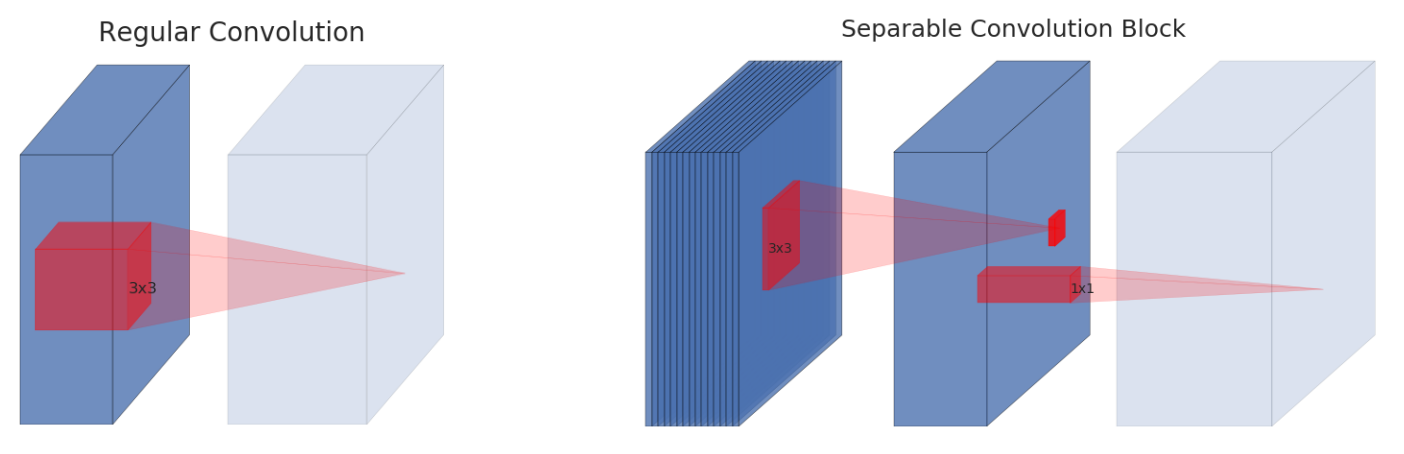
\includegraphics[width=0.6\textwidth]{images/Depthwise_Separable_Convolution.png}
    \caption{Depthwise Separable Convolution from \cite[Page 3]{sandler2018mobilenetv2} \newline On the left,
     a regular convolution with a 3x3xDepth kernel is drwan. On the right, this
     convolution is separated in depthwise convolution with a 3x3x1 Kernel,
     followed by a pointwise convolution with a 1x1xDepth Kernel. This methods
     saves computation time over the standard method, while also allowing
     interactions between channels.}
\end{figure}


With the second iteration called MobileNetV2 \cite{sandler2018mobilenetv2}, they
added the concept of inverted residuals or as they call it bottlenecks. The
ideas is, that intermediate representations should be low rather than high
dimensional. The bottleneck layer starts with a matrix with a small number of
depth channels. In the first step, the representation is expanded by a pointwise
convolution, followed by a Relu6. The expansion factor here controls how much
channels the intermediate representation will have. Then a depthwise convolution
is applied as an transformation step, followed again by a Relu6. Finally, a
pointwise convolution is applied again, but this time without a nonlinear
transformation following afterwards. The idea is that when compressing the data
back to a low dimensional space, a nonlinearity would only lead to a loss of
information. Finally, a skip connection from the input to the output is applied
to get a residual mapping from input to output.

For ImageNet, MobileNetV2 reaches an top-1 accuracy of 72\%, which outperforms
the competitors like MobileNetV1 or ShuffleNet 1.5 while having a similar number
of parameters.


\begin{figure}[h]\label{fig:InvRes}
    \centering
    \includegraphics[width=0.6\textwidth]{images/Inverted_Residual.png}
    \caption{Inverted Residual Block from \cite[Page 3]{sandler2018mobilenetv2}\newline 
    First, a Relu 6 followed by a Pointwise Convolution is applied to map the
     data to a higher dimensional space. Then a depthwise convolution is
     applied, followed again by a Relu6. Finally, the data is compressed back to
     the original size. This time, there is no Relu applied to avoid the loss of
     information.}
\end{figure}


\subsection{Network hyperparameters and training loop}\label{sub:Hyperparameters}
For both networks, the base hyperparameters are the same. Note that these
parameters are only standard configurations and may be changed to investigate
the effects:
\begin{itemize}
    \item Optimization Algorithm \\Stochastic Gradient descent combined with
    Momentum is used. A $\lambda$ of 0.9 is set for Momentum.
    \item Learning rate \\Initially 1e-2
    \item Batch size \\128
    \item Regularization \\An $L_2$ Regularization as described in chapter
    \ref{sub:Generalization} is used with a factor of 1e-3.
    \item Loss Function \\Cross-Entropy Loss
    \item Number of epochs \\The number of epochs varies. As this is an
    explorative analysis, the training is often run for a large number of
    epochs, to investigate long term changes. Usually an epoch number of 600 is
    used.
\end{itemize}

